%\clearpage
\section{Etat de l'art}
\label{sec:SOTA}

Dans le cadre de cette thèse, nous cherchons dans un premier temps à lier la dynamique des articulations d'un piéton à une intention. Cette estimation de la dynamique des articulations sera ensuite combinée à la vision afin d’avoir une estimation plus robuste et absolue de l'intention du piéton en fonction de son environnement.

\textit{De ce fait, nous avons du nous intérésser à plusieurs étapes indissociables}
\textit{De ce fait, nous avons du nous intérésser à plusieurs étapes qui seront considérées comme des parties indépendantes de notre approche}

\textit{3D action recognition – analysis of human actions based on3D  skeleton  data  –  becomes  popular  recently  due  to  its  succinctness,robustness, and view-invariant representation}

PipeLine: SQUELETTE -> HAR -> INTENTION

\subsection{Squelettisation de piétons}
La nécéssité première de cette thèse consiste donc en l'obtention d'une squelettisation cohérente de chaque piéton présent dans l'image au fil du temps.

Cette squelettisation sera ensuite utilisée en tant que donnée d'entrée de notre réseau afin d'en inférer une classe en fonction de la gestuelle de celui-ci.

L'idée de restreindre la gestuelle d'une personne à la seule évolution de son ossature au fil du temps n'est pas nouvelle.

Durant les années 70, les travaux en psychologie de Johansson  \cite{johansson1973visual,johansson1976spatio} ont permis de montrer qu'avec seulement des points lumineux, l'être humain interprétait facilement les stimulis qui lui étaient présentés comme ceux d'un être humain effectuant des actions: l'humain peut donc reconnaitre une action juste avec la pose et sans information annexe telle que l'environnement. 

\begin{figure}[H]
    \centering
    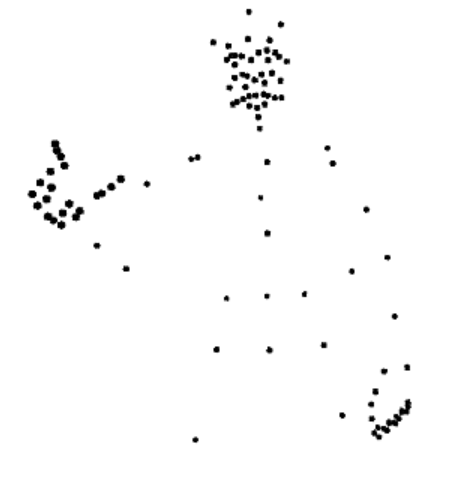
\includegraphics[width=0.34\linewidth]{Images/Johansson.png}
    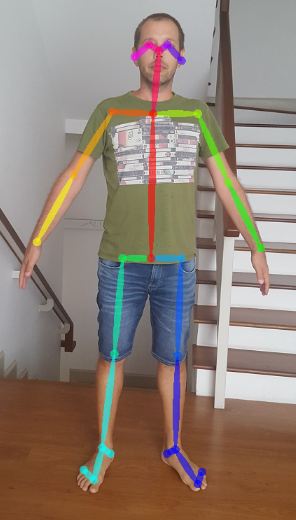
\includegraphics[width=0.2\linewidth]{Images/openpose2.png}
    \caption{A gauche: Un exemple de stimuli de l'experience de Johansson \cite{johansson1973visual,johansson1976spatio}.\\ A droite: la squelettisation obtenue après l'application d'Openpose \cite{cao2017realtime}}
    \label{fig:Johansson}
\end{figure}

La tâche de détection est compliquée par la variabilité de l’apparence des personnes (vêtements, pose ...)
ainsi que par des phénomènes d’occlusions, dûs à la foule et au décor ou encore dûs à des problèmes d'echelle dans l'image.




\label{subsec:SQUEL}
\subsubsection{Approches Top Down}
\subsubsection{Approches Bottom Up}

\subsection{Human Action Recognition}

\textbf{ Compared to RGB videos and optic flow,skeleton sequences are computationally efficient. Furthermore,skeleton  sequences  have  a  better  ability  to  represent  dataset-invariant  action  information  since  no  background  context  isincluded.
Parler des handcrafted?}

Les principales modalités utilisées pour la reconnaissance d'actions humaines comprennent les vidéos RGB dans leur globalité \cite{donahue2015long,2014arXiv1412.0767T,varol2017long,Wu_2018_CVPR}, le flow optique \cite{simonyan2014two,zhang2016real,sevilla2018integration,DanutPOP} et la réprésentation sous forme de squelette \cite{vemulapalli2014human,du2015hierarchical,2016arXiv160707043L,2018arXiv180107455Y}.

En réduisant la taille des données d'entrée grâce à la structure de données associée aux squelettes, ce type d'approche est considéré comme bien plus rapide computationellement parlant.

\label{subsec:HAR}

\subsubsection{Image-Based}
\subsubsection{Recurent neural network based}
\subsubsection{Graph Based}

\subsection{Intention Prediction}
\textit{La plupart des approches actuelles de la prédiction de l'action des piétons sont basées sur la trajectoire [16, 1, 5], ce qui signifie qu'elles s'appuient sur le mouvement passé observé des piétons et/ou la dynamique des véhicules pour prédire l'emplacement futur des piétons. Ces approches sont toutefois efficaces lorsque les piétons traversent déjà laa rue ou sont sur le point de le faire, c'est-à-dire que ces algorithmes réagissent à une action déjà en cours au lieu de l'anticiper.}

Un remède aux inconvénients courants des algorithmes basés sur la trajectoire est d'anticiper l'action en estimant sa cause ou son intention non déviante.


In the literature various terms such as intention, actionand behavior are used to describe what the agent is doing or about to do in the scene. Here, we distinguish intention as the underlying state of mind which cannot be observed but can be inferred from the behavior. This is opposed toactions and, more generally, behaviors, i.e. observable ac-tions such as walking or crossing, for which there is groundtruth available.




\subsubsection{Handcrafted}
\subsubsection{Apprentissage profond}


